
\section{Sampling Process}

\begin{figure}[h]
	\centering
	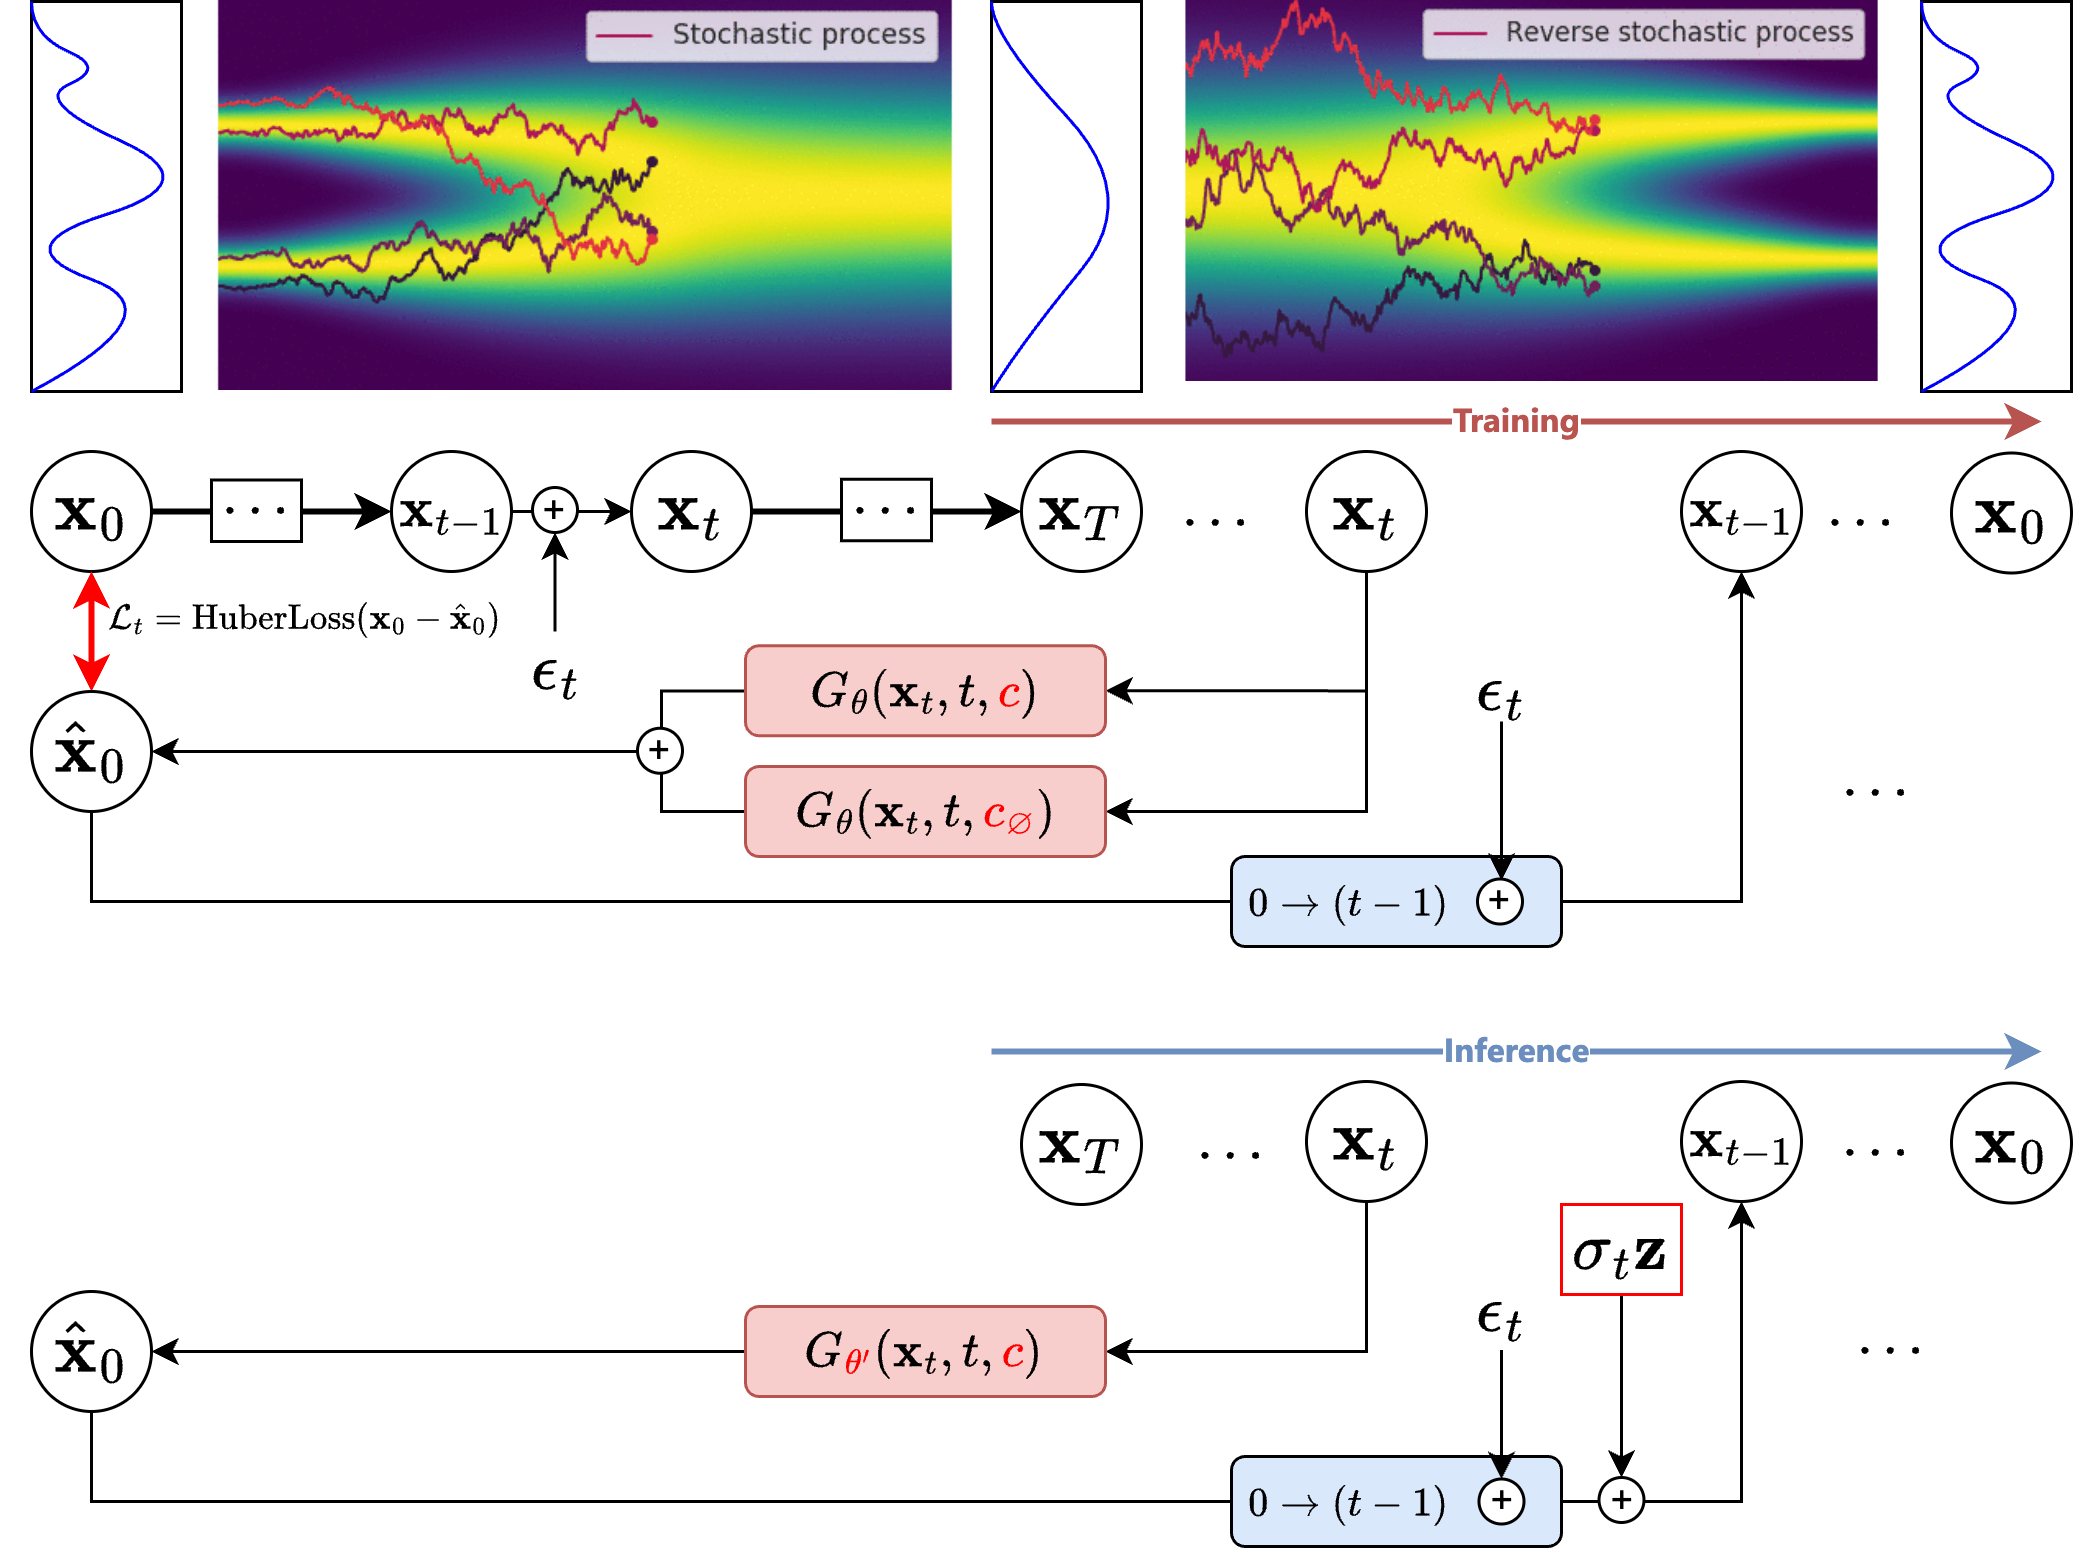
\includegraphics[width=\linewidth]{figures/OnlineAndOffline}
	\caption{Offline (Training) and Online (Inference) Phases}
	\label{fig:OnlineAndOffline}
\end{figure}

\vspace{-5mm}

To generate gestures of arbitrary length, the original sequence is segmented into clips of length $M$.
During training, the seed gesture can be chosen by randomly selecting a gesture from the dataset or by averaging the clipped segments-here, the mean rotation angles are used.  
Generated frames are processed sequentially, with the last $N=8$ frames taken as the seed for the next iteration.  
For each clip, the gesture $\bx_{t}$ is denoised via $\hat{\bx}_{0} = G_{\theta'}(\bx_{t}, t, c)$; noise is re-added to obtain $\bx_{t-1}$, and the procedure repeats until $t=1$, yielding $\bx_{0}$.

\begin{algorithm}[h]
	\caption{Sampling in DeepGesture}
	\label{alg:sampling}
	\setlength{\baselineskip}{10pt}
	\begin{enumerate}
		\item Initialize with noise: $\mathbf{x}_T \sim \mathcal{N}(0, \mathbf{I})$.
		\item Retrieve $\sqrt{\alpha_t}$, $\sqrt{1 - \alpha_t}$, and $\sqrt{\bar{\alpha}_t}$ from training; precompute $\sigma_t$ from $\alpha_t$ for each timestep $t: 1 \rightarrow T$.
		\item Split each 4-second speech segment into $\mathbf{a} \in \mathbb{R}^{64000}$.  
		The initial seed gesture $\mathbf{s}$ is the data mean and later updated from the inferred gesture segment.  
		Select the desired emotion, obtain the transcript $\mathbf{v}$ from speech $\mathbf{a}$, and form the condition $c = [\mathbf{s}, \mathbf{e}, \mathbf{a}, \mathbf{v}]$.
		\item For each timestep, take $t$ \textbf{sequentially} from $[T, \dots, 1]$.
		\item Sample random noise $\mathbf{z} \sim \mathcal{N}(0, \mathbf{I})$.
		\item Infer $\hat{\mathbf{x}}_0^{(t)} = G_{\theta'}(\mathbf{x}_t, t, c)$.
		\item Diffuse $\hat{\mathbf{x}}_0^{(t)}$ from step $0 \rightarrow t$ to obtain $\hat{\mathbf{x}}_{t-1}^{(t)}$.
		\item Add noise: $\hat{\mathbf{x}}_{t-1} = \hat{\mathbf{x}}_{t-1}^{(t)} + \sigma_t \mathbf{z}$.
		\item Return to step 4.  
		When $t = 1$, output the denoised gesture $\hat{\mathbf{x}}_0$.
	\end{enumerate}
\end{algorithm}


\autoref{alg:sampling} starts by initializing the noisy gesture $\mathbf{x}_T$ from $\mathcal{N}(0, \mathbf{I})$.  
The values $\sqrt{\alpha_t}$, $\sqrt{1-\alpha_t}$, and $\sqrt{\bar{\alpha}_t}$ obtained during training, together with $\sigma_t$, are employed at each timestep (1 … $T$).  
Each 4-second speech segment is represented by $\mathbf{a}$, and the seed gesture $\mathbf{s}$ is taken as the data mean or from the previously inferred segment.  
The desired emotion and the transcript form the condition $c = [\mathbf{s}, \mathbf{e}, \mathbf{a}, \mathbf{v}]$.  
The algorithm proceeds sequentially from $T$ to 1: random noise $\mathbf{z}$ is generated, the model predicts $\hat{\mathbf{x}}_0^{(t)}$ from $\mathbf{x}_t$, $t$, and $c$, then $\hat{\mathbf{x}}_{t-1}^{(t)}$ is computed and perturbed with noise.  
This loop continues until $t=1$, after which the algorithm outputs the final denoised gesture $\hat{\mathbf{x}}_0$.
